\documentclass{article}

% if you need to pass options to natbib, use, e.g.:
% \PassOptionsToPackage{numbers, compress}{natbib}
% before loading nips_2016
%
% to avoid loading the natbib package, add option nonatbib:
% \usepackage[nonatbib]{nips_2016}

\PassOptionsToPackage{numbers,sort&compress}{natbib}
\usepackage[final]{nips_2016} % produce camera-ready copy

\usepackage[utf8]{inputenc} % allow utf-8 input
\usepackage[T1]{fontenc}    % use 8-bit T1 fonts
\usepackage{hyperref}       % hyperlinks
\usepackage{url}            % simple URL typesetting
\usepackage{booktabs}       % professional-quality tables
\usepackage{amsfonts}       % blackboard math symbols
\usepackage{nicefrac}       % compact symbols for 1/2, etc.
\usepackage{microtype}      % microtypography
\usepackage{graphicx}
\usepackage{float}
\usepackage{hyperref}
\usepackage{amsmath}
\usepackage{bbm}
\usepackage{dsfont}
\usepackage{multirow}
\usepackage{multicol}
\usepackage{subcaption}

\title{Species Distribution Modeling of Presence-only Species Data}

% The \author macro works with any number of authors. There are two
% commands used to separate the names and addresses of multiple
% authors: \And and \AND.
%
% Using \And between authors leaves it to LaTeX to determine where to
% break the lines. Using \AND forces a line break at that point. So,
% if LaTeX puts 3 of 4 authors names on the first line, and the last
% on the second line, try using \AND instead of \And before the third
% author name.

\author{
  s2602238\\
  %% examples of more authors
  \And
  s2531687\\
 \And
  s2535212\\
}

\begin{document}

\maketitle

\begin{abstract}
 Species distribution modeling (SDM) plays a pivotal role in ecological research and conservation initiatives, offering valuable insights into the spatial distribution of species. This report is dedicated to addressing the challenges associated with positive-only data, commonly known as presence-only data, within the realm of SDMs. Our approach compares different loss functions that address the issue of presence-only data. The primary objective is to tackle the limitations posed by datasets that only provide information about the presence of a species without explicit confirmation of absence. Employing machine learning models, we predict the presence or absence of species in a given geographic location. Specifically, we implemented a multi-species model, leveraging the capabilities of a neural network and several different loss functions. The weak assume negative (WAN) loss function and our up-weighting positive label (UPL) loss function allowed the neural network to improve significantly over the binary cross-entropy loss function in various metrics. 
\end{abstract}

\section{Introduction}
Species distribution modeling (SDM) is indispensable in ecology and conservation biology for predicting and understanding the spatial distribution of organisms in geographic space \cite{review, rareplants}. More specifically, species distribution modeling is the process of using species observation records to develop a statistical model for predicting whether a species is present or absent at any location \cite{spatial}. In the broader context of biodiversity conservation, SDMs serve as helpful tool that provide valuable insights into habitat preferences and aide in the strategic allocation of resources for effective preservation efforts.

Species distribution modeling relies on species observation data, which can be categorized into presence-only and presence-absence data. Presence-only data refers to information indicating the occurrence of a phenomenon only where it is observed, while presence-absence data includes information on both the presence and absence of the phenomenon across locations. Presence-only data is readily available and more easily collected, whereas presence-absence data is less common due to challenges associated with verification of absences \cite{spatial, review, presence-onlyEM}. Given the significance of being able to effectively leverage the substantial supply of presence-only data, this report focuses on training a model with presence-only data. 

There are a wide variety of models used in species distribution modeling, each having their own use case. In the category of presence-only data, the most common approach is using the maximum entropy method (MaxEnt). The MaxEnt model, as described in \cite{review, maxent, rareplants}, estimates the probability of observing a species based on environmental covariates, ensuring consistency with observed species data and minimizing Kullback-Leibler divergence to closely match the marginal distribution of the covariates. Other models that are commonly used with presence-only data include boosted regression trees, random forests, support vector machines, and neural networks \cite{multi-speciesembedding, review, cnnenvironmentcooccurrences}. Our experiments employ a neural network to tackle the challenge posed by presence-only data by leveraging various loss functions. Neural networks, recognized for their ability to capture intricate relationships, have gained prominence as effective models in species distribution modeling.

\section{Data preparation}

\subsection{Sinusoidal Encoding}

Our dataset is described such that $\mathbf{x}$ = [\text{lon}, \text{lat}] denotes a geographical location (the longitude and latitude of the location). The sinusoidal encoding method is applied to normalize and encode the geographical coordinates, transforming longitude and latitude into a sinusoidal representation. This approach effectively captures the cyclic nature of these coordinates. The process involves first normalizing each longitude and latitude value to a range between -1 and 1. Subsequently, following \cite{spatial, colecomputervision}, each coordinate is encoded into a pair of sine and cosine values. This results in a 4-dimensional encoded vector for each location, represented as \( \mathbf{x} = \left[ \sin(\pi \cdot \text{lon}), \cos(\pi \cdot \text{lon}), \sin(\pi \cdot \text{lat}), \cos(\pi \cdot \text{lat}) \right] \).

\subsection{One Hot Encoding} One-hot encoding is applied to transform the species labels into a binary one-hot encoded vector (vector of labels $\mathbf{z}$ from the label space $\mathbf{Z} = \{0, 1\}^L$) where each index corresponds to a unique species ID. If a specific species is present at a location, the corresponding index in the vector is set to 1; otherwise, it's set to 0. The first step of one-hot encoding is to identify all the unique labels (species) present in the categorical feature.  After identifying the unique categories, a binary vector for each of unique categories is created. This binary vector is the same length as the total number of unique categories. In this binary vector, 1 indicates the presence of the species, while 0s indicate the absence. 

\section{Exploratory Data Analysis}

The iNaturalist dataset contains the geospatial distribution of animal sightings and prevalence. In the data there are 500 different species and a total of 272,037 observation locations. On average, each species is associated with approximately 544 observation locations, with the minimum number of locations for a species being 50 and the maximum reaching 2,000 locations. The iNaturalist data was collected through crowdsourcing the features from an online community. iNaturalist serves as both a crowdsourced species identification system and an organism occurrence recording tool. The majority of the species have less than 500 occurrences in the dataset. This means that our classes are unbalanced and we have some species with a larger number of locations in the test dataset. Only a small portion of the species have 2000 observations.

In Figure \ref{fig:worldheatmap} we can see the density of our observations plotted over the the world map using the longitude and latitude values of the training dataset. We can see that the density is higher in North America and Australia, with the other continents having less density. 

% \begin{figure}[H]
%     \centering
%     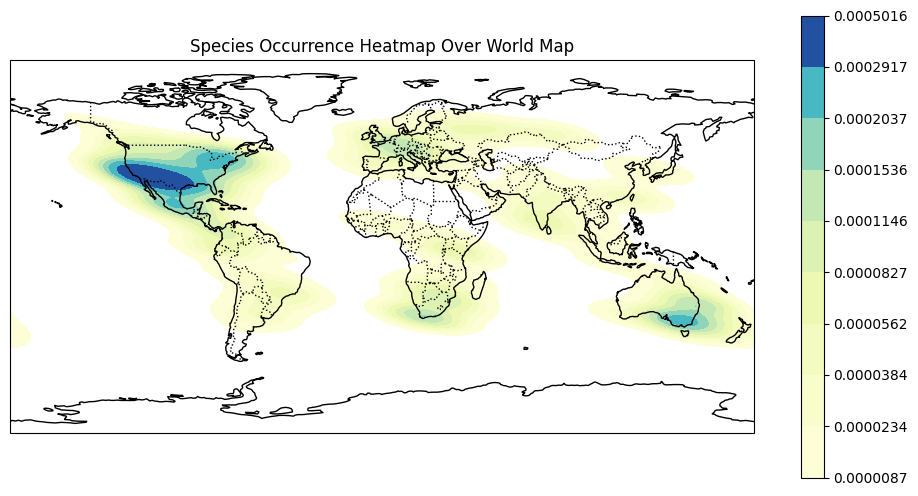
\includegraphics[width=1\linewidth]{heatmap_world_map.png}
%     \caption{Heatmap of species occurrences on the world map}
%     \label{fig:worldheatmap}
% \end{figure}

\begin{figure}[H]
    \centering
    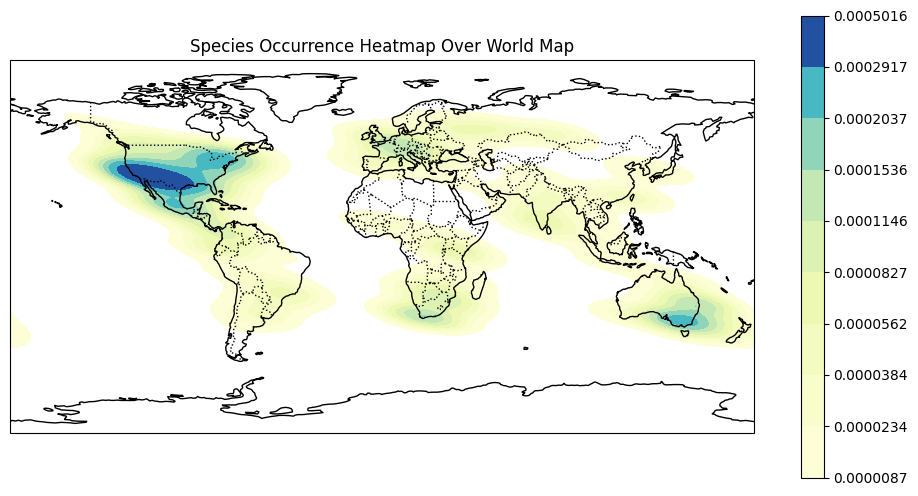
\includegraphics[width=1\linewidth, height=0.25\textheight]{heatmap_world_map.png}
    \caption{Heatmap of species occurrences on the world map}
    \label{fig:worldheatmap}
\end{figure}


\section{Methods}
In a standard multi-class classification problem, each $\mathbf{x}$ (input data vector) from the input space $\mathbf{X}$ is assigned to a single label from $\{1, \ldots, L\}$, where $L$ is the number of classes. In the multilabel classification setting, each $\mathbf{x}$ is associated with a vector of labels $\mathbf{t}$ from the label space $\mathbf{T} = \{0, 1\}^L$, where an entry $t_{n} = 1$ if the $n$th class is associated to $\mathbf{x}$ and $t_{n} = 0$ if the $n$th class is not associated to $\mathbf{x}$ \cite{cole2021multilabel}. Our case is the multilabel classification setting. 

Our dataset is described such that $\mathbf{x}$ = [\text{lon}, \text{lat}] denotes a geographical location (the longitude and latitude of the location). Let $\mathbf{t} \in \{0, 1\}^L$ denote the true presence (1) or absence (0) of $L$ different species at location $\mathbf{x}$. Here 
$\mathbf{t}$ denotes the fully observed label vector. However, our dataset is such that we don't have access to this fully observed label vector and instead are working with $\mathbf{z_{n}} \in \mathcal{\mathbf{Z}} = \{0, 1, \emptyset\}^L$, where $z_{ni} \in \{0, 1\}$ can be described as before and where $z_{ni} = \emptyset$ indicates that the $i$-th label is unobserved for $\mathbf{x_n}$. This means that if $z_{ni} = \emptyset$, then the corresponding $t_{ni}$ could be either 0 or 1. This is the known as partially observed setting \cite{spatial,cole2021multilabel}.

To summarize, $\mathbf{z} \in \{0, 1, \emptyset\}^L$ represents our observed data at $\mathbf{x}$, where $z_j = 1$ if species $j$ is present, $z_j = 0$ if species $j$ is absent, and $z_j = \emptyset$ if we do not know whether species $j$ is present or absent. The model produces an estimate of $\mathbf{t}$ at any location $\mathbf{x}$ over the input space $\mathbf{X}$, given observed data $\{(\mathbf{x_i},\mathbf{z_i})\}_{i=1}^N$. The predictions are given by $\mathbf{{y}} = h(f_\theta(\mathbf{x}))$, where $f_\theta$ is a multi-layer neural network with parameters $\theta$ and $h$ is a layer which applies sigmoid function to each values given by our multi-layer neural network. The prediction $\mathbf{{y}} \in [0, 1]^L$ represents our estimate of how likely each species is to be present at $\mathbf{x}$.


Our scenario falls on a particular case of the partially observed setting which is called the \emph{single positive only case}, where we observe one single positive label per training example, and all the other labels are unknown. This 'single positive only' instance here refers to having presence-only data. This can be represented mathematically as :

$z_{ni} \in \{1, \emptyset\}$ for all $n \in \{1, \ldots, N\}$, $i \in \{1, \ldots, L\}$.

$\sum_{i=1}^L I[z_{ni}=1] = 1$ for all $n \in \{1, \ldots, N\}$, where  I[.] denotes the indicator function \cite{cole2021multilabel}

\subsection{Presence-only Data}

Ideally, in species distribution modeling, the most comprehensive dataset would consist of presence-absence data, capturing locations where a species has been observed to be present as well as locations where it has been confirmed to be absent. Having confirmed information about where a species is present and where it is absent enables a more robust characterization of its habitat preferences. Presence-absence data, although significantly more desireable, is also significantly more difficult to obtain and is often not even available~\cite{review,AcknowledgingMultilabelSPLZhou}. The practicality of obtaining presence-absence data at scale is constrained by the logistical challenges and costs associated with confirming absences. Confirming absence necessitates the deployment of skilled observers to conduct exhaustive searches, making comprehensive presence-absence datasets difficult to obtain, particularly for large-scale studies \cite{spatial}.

In contrast, the more prevalent scenario is the use of presence-only data, where the focus is solely on locations where a species has been observed to be present, and absences are not explicitly confirmed. The data from iNaturalist falls under this category. Presence-only data is more abundant and easier to acquire, making it a practical choice when faced with resource constraints. However, the lack of confirmed absence information in presence-only datasets introduces challenges in capturing the complete ecological range of a species. The trade-off between the richness of presence-absence data and the practicality of acquiring presence-only data underscores the complexities researchers face when constructing datasets for species distribution modeling. 

\subsection{Multilabel Classification}

To mitigate the challenge associated with presence-only data, we examined the loss functions applicable to two different scenarios: fully observed labels and positive-only labels. For fully observed labels, we are using the binary cross-entropy loss (BCE), and then we look into how the BCE loss is altered for the positive-only label case. BCE loss is a frequently utilized and simple multi-label loss function. We denote our vector of predictions for an input vector $\mathbf{x_{n}}$ as $\mathbf{y_{n}} \in \{0, 1\}^L$, where $y_{ni}$ denotes the ith entry of $\mathbf{y_{n}}$.

    
\subsubsection{Fully Observed Labels}

For a fully observed data point ($\mathbf{x_{n}}$,$\mathbf{t_{n}}$), the BCE loss is described as the following:

\[
L_{BCE}(\mathbf{y}_n, \mathbf{t}_n) = \frac{1}{L} \sum_{i=1}^{L} \left[ t_{ni} \cdot \log(y_{ni}) + (1 - t_{ni}) \cdot \log(1 - y_{ni}) \right]
\]

where $\mathbf{t}_n$ represents the fully observed label vector.
\subsubsection{Positive only Labels}

Suppose that we have partially observed data $(\mathbf{x_n, z_n)}$, and suppose that all of the observed labels are positive, i.e., $z_{ni} = \emptyset \implies z_{ni} = 1$. The most straightforward strategy is to assume unobserved labels as negative, i.e., $z_{ni} = 0$ if $z_{ni} = \emptyset$. The resulting "assume negative" (AN) loss is given by the following \cite{cole2021multilabel} :
\begin{equation}
    L_{AN}(\mathbf{y}_n, \mathbf{z}_n) = -\frac{1}{L} \sum_{i=1}^{L} [z_{ni} \cdot \log(y_{ni}) + (1 - z_{ni}) \cdot \log(1 - y_{ni})].
\end{equation}

The drawback is that this assume negative approach will introduce some number of false negatives.

\subsubsection{Weak Assume Negatives}

A simple way to mitigate the impact of false negatives is to down-weight the terms in the loss which corresponds to negative labels. For this, we use a parameter $\gamma \in [0, 1]$, and hence the resulting "weak assume negative" (WAN) loss is defined as the following \cite{cole2021multilabel} : 
\begin{equation}
    L_{WAN}(\mathbf{y}_n,\mathbf{z}_n) = -\frac{1}{L} \sum_{i=1}^{L} [z_{ni} \cdot \log(y_{ni}) + (1 - z_{ni}) \cdot \gamma \cdot \log(1 - y_{ni})].
\end{equation}

we choose $\gamma = \frac{1}{L-1}$, so that the single positive label has the same influence on the loss as the $L-1$ assumed negatives labels.

\subsubsection{Up-weighting the positive labels}

Another approach to mitigate the impact of false negatives is to up-weight the term in the loss function which corresponds to positive label. For this we use a parameter  $\alpha$ which is greater than 1, and hence the resulting "up-weighting positive label" (UPL) loss is defined as the following:

\begin{equation}
    L_{UPL}(\mathbf{y}_n,\mathbf{z}_n) = -\frac{1}{L} \sum_{i=1}^{L} [z_{ni} \cdot \log(y_{ni})\cdot\alpha + (1 - z_{ni}) \cdot \log(1 - y_{ni})]
\end{equation}

Again, we choose $\alpha = {L-1}$ such that the single positive label has the same influence on the loss as the $L-1$ assumed negatives labels.
\subsection{Network Architecture}
The neural network architecture that was implemented for our SDM is comprised of an input layer with 4 features, followed by four hidden layers with 32, 64,128 and 200 neurons respectively. These layers are interconnected by linear transformations, ReLU activation and finally we apply Sigmoid activation at the output of the last layer. These functions enable the network to model complex data patterns effectively. Adam optimizer facilitates efficient gradient-based optimization during training. The network is trained for 150 epochs. The choice of architecture allows the model to process information from the 4 input features and gradually extract increasingly complex features through the hidden layers, providing the capacity to capture intricate patterns and relationships within the data. These hyperparameters were selected following multiple iterations and experimentation.

\section{Results}

In order to measure the performance of our model, we must consider a number of metrics. The evaluation SDMs has been a known difficulty. In the context of machine learning, the usual method involves making predictions on a separate set of data and assessing performance using a relevant metric; however, the major issue is determining what the ground truth is \cite{review}. Although our training data is presence-only, we have a test set that includes the locations for all species from the training set and for each location we know if a species is present there or not. Typically this type of test set is unavailable and having the presence-absence data will make evaluation much more straightforward. Even with the available test set, observations inherently contain some degree of noise. Confirming the absence of a species in an area is particularly challenging and can only be done with a certain level of certainty \cite{review}. In this section we will review a few different metrics that show our model's performance.  

\subsection{ROC Curve and AUC}
The Receiver Operator Characteristic (ROC) approach, specifically the Area Under the ROC Curve (AUC), is commonly used to assess the accuracy of probabilistic output models in species distribution modeling \cite{moutonEcologicalRelevancePerformance2010, rareplants, maxent}. The ROC curve is a graph depicting a classification model's performance at various thresholds by plotting True Positive Rate (TPR) against False Positive Rate (FPR). 

\begin{equation*}
\begin{aligned}
TPR & = \frac{\text{True Positives}}{\text{True Positives + False Negatives}}, & \quad
FPR & = \frac{\text{False Positives}}{\text{False Positives + True Negatives}}
\end{aligned}
\end{equation*}


AUC is a single scalar value, ranging from 0 to 1, that quantifies a model's overall performance. It represents the integral of the ROC curve. A higher AUC indicates better discrimination between positive and negative instances.


\subsection{Precision, Recall, F1-score}

The formulas for precision, recall, and F1-score are the following: \[ P = \frac{TP}{TP + FP}, \quad R = \frac{TP}{TP + FN}, \quad F1 = \frac{2 \cdot P \cdot R}{P + R} \]

where \(TP\) is the number of true positives, \(FP\) is the number of false positives, and \(FN\) is the number of false negatives. Precision measures the percentage of the items that the system detected that are in fact positive, recall measures the percentage of items actually present in the input that were correctly identified by the system, and the F1-score provides a balanced measure by considering both precision and recall. These metrics are particularly crucial in scenarios where different classes have varying frequencies. In our case, we have data where there are large differences in class frequencies, as we can see in Figure \ref{fig:speciesbarchart}. In the context of multi-class classification, micro-averaging aggregates decisions across all classes into a single confusion matrix and computes precision and recall. Macro-averaging computes performance for each class separately and then averages over classes. We use both these metrics to show the overall performance. The micro-average is dominated by the more frequent class, since the counts are pooled, and the macro-average better reflects the statistics of the smaller classes \cite{jm3}. 







\subsection{Jaccard and Hamming Score}
Jaccard Score is a measure of similarity between two sets. In our evaluation, it is applied to assess the overlap and agreement between the predicted labels and the true labels for a given sample or data point. The Jaccard Score ranges from 0 to 1, where 0 indicates no overlap (complete dissimilarity), and 1 represents perfect overlap (complete similarity). \\
The Hamming Score, on the other hand, is a metric used to assess the accuracy of multi-label classification models. It measures the proportion of correctly predicted labels to the total number of labels.

\subsection{Final Results}
\begin{table*}[h]
    \centering
    \begin{tabular}{c|c|cccc}
    \toprule
        Model    &  Average measure & Precision & Recall & F1 Score & Jaccard Score \\
    \midrule
    \midrule
        \multirow{2}*{Baseline (BCE Loss)}
                 & micro avg                 &  0.0                &      0.0 & 0.0 & 0.0 \\
                 & macro avg  & 0.0 & 0.0 & 0.0  & 0.0 \\
    \midrule
        \multirow{2}*{Implementing WAN Loss }
                 & micro avg                 &   0.23              &      0.77 & 0.35 & 0.21 \\
                 & macro avg  & 0.19 & 0.74 & 0.27 & 0.17     \\
    \midrule
        \multirow{2}*{Implementing UPL Loss}
                 & micro avg                 &  0.24              &  0.78 & 0.36    & 0.22 \\
                 & macro avg  & 0.18       & 0.74       & 0.26  & 0.17   \\  
    \bottomrule
    \end{tabular}
    \caption{Evaluation Metrics}
    \label{tab:hp_search}
\end{table*}

\begin{table*}[h]
    \centering
    \begin{tabular}{c|c|c}
    \toprule
        Model    & Hamming accuracy& Area under ROC Curve \\
    \midrule
    \midrule
        Baseline & 98.8 & 0.5 \\
        WAN & 96.6 & 0.86 \\
        UPL & 96.7 & 0.85 \\
    \bottomrule
    \end{tabular}
    \caption{Additional Metrics}
    \label{tab:additional_metrics}
\end{table*}

Our baseline model, employing the standard Binary Cross Entropy (BCE) loss, yields an Area Under the Receiver Operating Characteristic (AUC-ROC) value of 0.5 as shown in \ref{fig:Baseline Model with standard BCE loss}. This signifies that the model's performance is no better than random chance in distinguishing between positive and negative instances. This limitation is attributed to fact that the model is attempting multi-label predictions during testing, despite being trained on instances with only one positive label during training.

Although the baseline model attains a high Hamming accuracy of 98.8, it records a value of zero in various other metrics such as precision, recall, F1 score, and Jaccard score. This discrepancy suggests challenges in accurately classifying individual labels within the multi-label classification task. The model tends to predict all instances as negative, leading to high Hamming accuracy but poor performance in label-specific metrics.

The models employing the "weak assume negative" loss and "up-weighting the positive label" loss strategically adjust the weights associated with negative and positive labels in the standard binary cross entropy loss. This effectively mitigates the impact of false negatives, resulting in improved values for metrics such as precision, recall, F1 score, and Jaccard score compared to the baseline model. Also these models achieve AUC-ROC values of 0.86 and 0.85, respectively as shown in \ref{fig:Model implementing the WAN loss} and \ref{fig:Model implementing the UPL loss}. These results indicate that these models perform reasonably well in distinguishing between positive and negative instances compared to a random classifier. 




\section{Conclusion}


We delved into the challenge of associating species with geographical locations through the utilization of multi-layer neural networks. During our investigation, we observed that our initial model, employing the standard Binary Cross-Entropy (BCE) loss, exhibited poor performance. This was attributed to the model attempting to make multi-label predictions during testing, despite encountering only one positive label per training instance. This issue, arising from Species Distribution Modeling (SDM) with presence-only data, can be conceptualized as a form of multi-label classification with incomplete supervision.

To address this, we experimented with two alternative models aimed at mitigating the impact of false negatives. The first involved down-weighting the terms associated with negative labels in the standard BCE loss, while the second up-weighted the term corresponding to the positive label. Both approaches yielded comparable metrics and significantly outperformed our baseline model across all evaluated criteria. However considering alternative methods like maximum entropy loss, which promotes maximizing entropy for predictions of unobserved labels rather than enforcing them to be zero, could offer even more improvement in evaluated metrics.


\newpage
\bibliography{refs.bib}
\bibliographystyle{plain}

\newpage

\appendix
\section*{\Large Appendices}
\section{Species Bar Chart}


\begin{figure}[H]
    \centering
    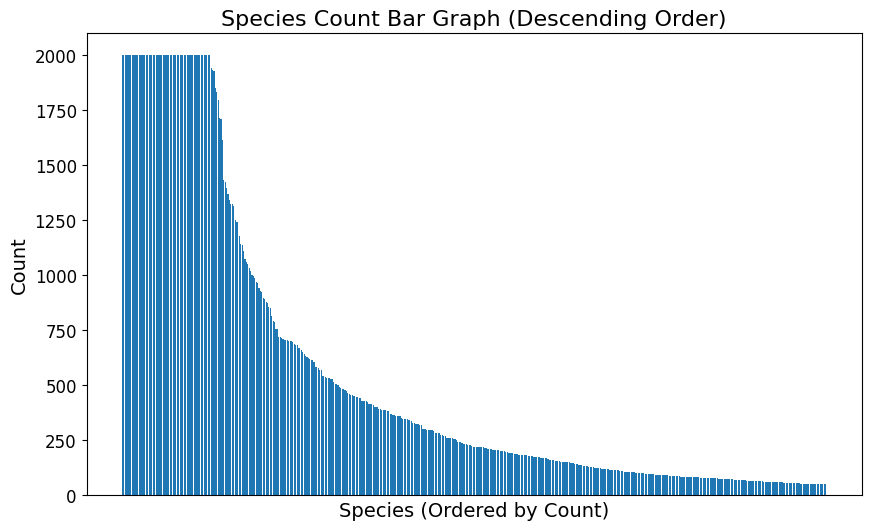
\includegraphics[width=1\linewidth]{speciesbarchart.png}
    \caption{Each species count of occurrences in descending order.}
    \label{fig:speciesbarchart}
\end{figure}

Figure \ref{fig:speciesbarchart} shows a tilted bar chart that represents the count of occurrences for each species, arranged in descending order of count. The graph is used to visually represent the frequency of each species within a dataset, with the most frequent species on the left and the least frequent on the right. This chart shows that most of the species have less than 500 locations. 



\section{Receiver Operating Characteristics}

Our baseline model, which uses the standard "binary cross entropy" loss, results in an Area Under the Receiver Operating Characteristic (AUC-ROC) value of 0.5 as shown in \ref{fig:Baseline Model with standard BCE loss} This indicates that the model performs no better than random chance in distinguishing between positive and negative instances. The model's ability to discriminate between the two classes is essentially equivalent to making random predictions. This is attributed to the fact that the model is attempting to make multi-label predictions during testing, despite encountering only one positive label per training instance.

Figures \ref{fig:Model implementing the WAN loss} and \ref{fig:Model implementing the UPL loss} represents how the models using the "weak assume negative" loss and "up-weighting the positive label" loss have AUC-ROC values of 0.86 and 0.85, respectively. This indicates that these models perform reasonably well in distinguishing between positive and negative instances compared to a random classifier.

\begin{figure}
    \begin{subfigure}{\textwidth}
        \centering
        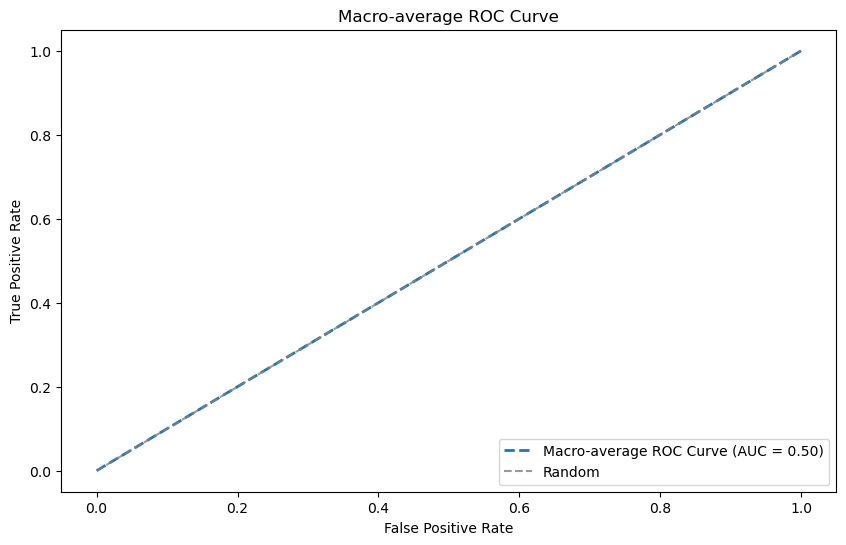
\includegraphics[width=0.75\linewidth]{BASELINE.png}
        \caption{Baseline Model with standard BCE loss}
        \label{fig:Baseline Model with standard BCE loss}
    \end{subfigure}

    \vspace{10pt} % Add some vertical space

    \begin{subfigure}{\textwidth}
        \centering
        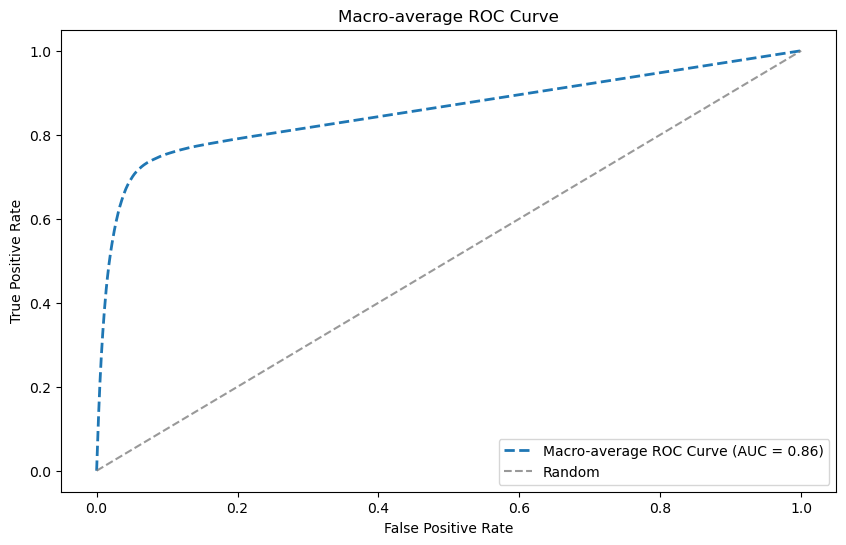
\includegraphics[width=0.75\linewidth]{Model with WAN.png}
        \caption{Model implementing the WAN loss}
        \label{fig:Model implementing the WAN loss}
    \end{subfigure}

    \vspace{10pt} % Add some vertical space

    \begin{subfigure}{\textwidth}
        \centering
        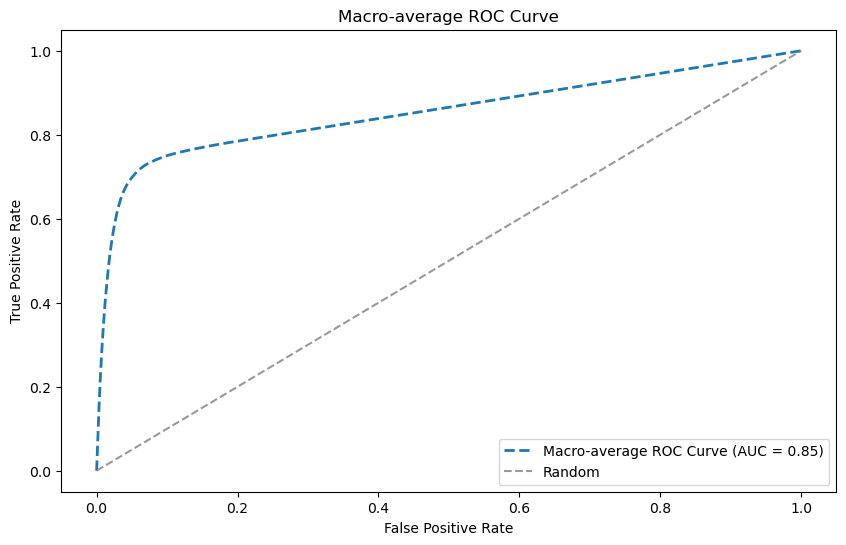
\includegraphics[width=0.75\linewidth]{Model with UPL.png}
        \caption{Model implementing the UPL loss}
        \label{fig:Model implementing the UPL loss}
    \end{subfigure}

    \caption{Comparison of different models}
    \label{fig:models_comparison}
\end{figure}

\section{Neural Network Diagram}

\begin{figure}[H]
    \centering
    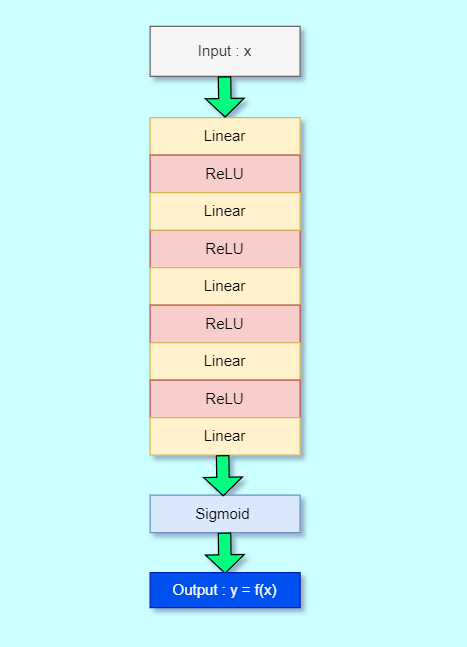
\includegraphics[width=0.6\linewidth]{Neural.png}
    \label{fig:enter-label}
\end{figure}

\textbf{Hyperparameters tuning} : 
Different activation functions were tested, namely the tanh, ReLU and a combination of tanh with ReLU. It was observed that the standalone use of ReLU yielded the best results.
also different learning rate for the adam optimiser was tested. It was found that a learning rate of 0.007 provided the most favorable outcome, striking a balance between efficient learning and the stability of the convergence process.

\section{Data Loading}
In this section, we outline the procedure for loading the training and testing data used in our experiments.

The training data, which is sourced from iNaturalist \cite{iNaturalist}, is comprised of presence-only information. The central components of the training dataset include two key arrays: \texttt{train\_locs}, a 2D array where each row represents a data point with columns indicating geographic coordinates (latitude and longitude); and \texttt{train\_ids}, a 1D array containing the species ID associated with each location in \texttt{train\_locs}. Additionally, the dataset provides a comprehensive list of specie IDs alongside their Latin names under the \texttt{species} and \texttt{species\_names} arrays, essentially forming a reference dictionary for the species identification.

The testing data, sourced from IUCN \cite{iucn}, is designed for presence-absence analysis. It consists of \texttt{test\_locs}, another 2D array representing geographic coordinates. A critical component is \texttt{test\_pos\_inds}, acting as a mapping mechanism that links species IDs to the indices in \texttt{test\_locs}, indicating the presence of specific species at these indexed locations.

These loading procedures establish the foundation for the subsequent analysis and model training in our experiments.

\section*{\Large Statement of Contribution}
\section*{s2602238}
Wrote the Python/PyTorch code for the baseline model implementing the standard "binary cross entropy" loss,  exploratory data analysis, evaluation metrics(Jaccard score, area under ROC curve) and contributed towards the writing of the overall report.
\section*{s2531687}
Wrote the Python/PyTorch code for the model implementing the "weak assume negative" loss ,  data preprocessing (sinusoidal encoding and one-hot encoding for train and test data) and contributed towards the writing of the overall report.
\section*{s2535212}
 Wrote the Python/PyTorch code for the model implementing the "up-weighting the positive label" loss, evaluations metrics (precision, recall, f1 score and hamming accuracy) and contributed towards the writing of the overall report.
 
\end{document}




%%% Local Variables:
%%% mode: latex
%%% TeX-master: t
%%% End:
